\documentclass[11pt]{article}
\title{\textbf{Meccano hexagons}}
\author{https://github.com/heptagons/meccano/hexa}
\date{}

\usepackage{amsmath}
\usepackage{listings}
\usepackage{xcolor}
\definecolor{gray}{RGB}{245,245,245}

\lstset{
	backgroundcolor=\color{gray},
	frame=single,
	language=c,
	numbers=left,
	stepnumber=1
}


\usepackage[margin=0.75in]{geometry}

\usepackage{tikz}
\usetikzlibrary{math}

\usepackage{graphicx}

\begin{document}

\maketitle

\section{Meccano hexagons}

\subsection {Regular diagonals}
A meccano hexagon can be build easily attaching sufficient equilateral
triangles as small as one unit side. 
Also joining six bars to form a perimeter and using two more rods as \textbf{regular diagonals},
which means both diagonals are aligned along the triangular grid.
Regular diagonals join opposite hexagon sides.

\begin{figure}[htpb]
\centering
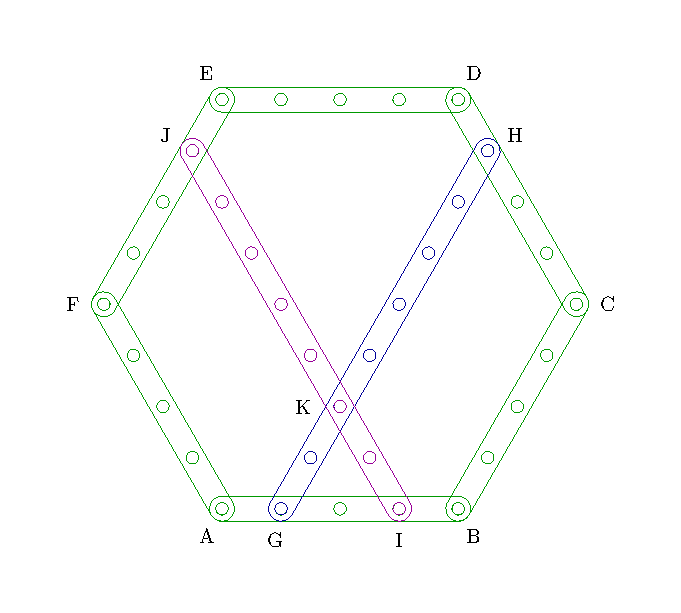
\includegraphics[scale=0.75]{hexagon_simple}
\caption{Hexagon of size $4$ with two \textbf{regular diagonals} of size $7$.}
\label{fig:regular}
\end{figure}

Consider figure \ref{fig:regular}.
Start with rod $\overline{AB}$ and add two rods $\overline{GH}$ and
$\overline{IJ}$ to form a triangle with three bolts at points $G$, $I$ and $K$. At this moment, perimeter points $A$, $B$, $H$ and $G$ are rigid.

Then add perimeter rods $\overline{BC}$ and $\overline{CD}$ with a bolt at $H$.
In the same way add perimeter rods $\overline{AF}$ and $\overline{EF}$ with a bolt at $J$.
At this moment everything is rigid. Finally add rod $\overline{DE}$ with bolts at $D$ and $E$.



\begin{figure}[htpb]
\centering
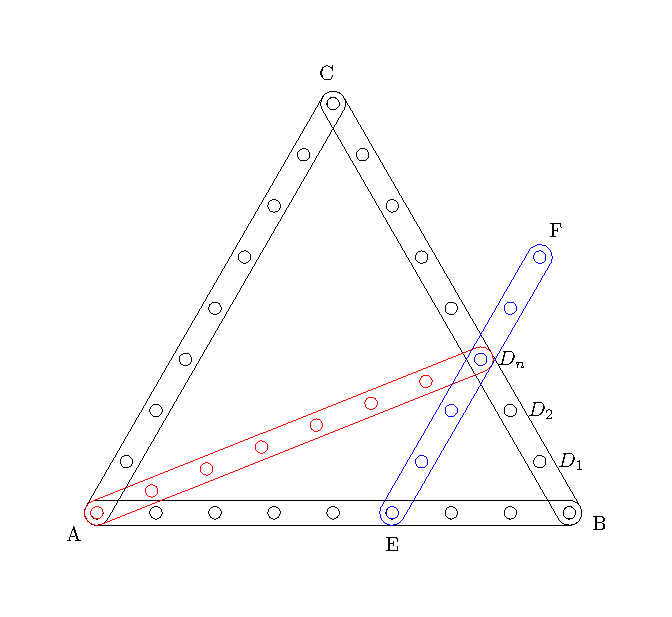
\includegraphics[scale=0.8]{hexagon_angle}
\caption{The red rod is an irregular diagonal, with integer length 
and joining two adjacent hexagon sides $\overline{AE}$ and $\overline{EF}$.}
\label{fig:irregular}
\end{figure}

\subsection{Irregular diagonals}

While regular diagonals are aligned along the triangular grid, \textbf{irregular diagonals}
don't. Irregular diagonals join two adjacent hexagon sides, making (rigid) irregular triangles.

Consider figure \ref{fig:irregular}.
Start with an equilateral triangle $ABC$ of side $\overline{AB}$.
Test one by one the irregular diagonals from the point $A$ to the points $D_1$, $D_2$..., $D_n$
which are over the rod $\overline{BC}$. Define the tree variables to use:
\begin{align*}
a &= \overline{AB}\\
b &= \overline{BD_n}\\
d &= \overline{AD_n}\\
\end{align*}
Acording to the cosines law and knowing the $\angle{EBD_n} = 60^\circ{}$, calculate $d$:
\begin{align*}
d &= \sqrt{a^2 + b^2 - 2ab\cos{\frac{\pi}{3}}}\\
  &= \sqrt{a^2 + b^2 - ab}\\
  &= \sqrt{(a-b)^2 + ab}\\
\end{align*}

Reject any non-integer diagonal $d$, since any meccano rod length should be an integer.
For the valid diagonal such as $\overline{AD_n}$, locate a point $E$ over the rod $\overline{AB}$
such so the distance $\overline{BE}$ equals the distance $\overline{BD_n}$.
From the point $E$ create a new rod $\overline{EF}$ passing over the point $D_n$ (blue rod in the figure).
Finally we got a valid \textbf{irregular diagonal} $d$ for the pair of adjacent
hexagon sides $\overline{AE}$ and $\overline{EF}$.

\subsection{Irregular diagonals program}

We need a program to iterate over integer $a$, then over integer $b$ to test whether $d$ value is an integer too.
Next golang program find the diagonals.
We iterate from $a=1$ to a given maximum (line 2).
Then we iterate from $b=1$ to $b <= a/2$ (line 3), to avoid repeating symmetric values.
In order to reject repetitions by scaling we check for greatest commond divisor
of $a$ and $b$ to be $1$ (line 4).
Then we calculate the diagonal using the formula $d^2 = (a-b)^2 + ab$ (line 5) and report
only the case when the diagonal is a square number (line 8). 
\begin{lstlisting}
func triangle_diagonals(max int) {
  for a := 1; a < max; a++ {
    for b := 1; b <= a/2; b++ {
      if gcd(a, b) == 1 {
        diag := (a-b)*(a-b) + a*b
        cd := math.Sqrt(float64(diag))
        d := int(cd)
        if cd == float64(d) {
          num := float64(diag + a*a - b*b)
          den := 2.0 * cd * float64(a)
          angle := 180*math.Acos(num/den)/math.Pi
          fmt.Printf("a=%3d b=%3d d=%3d angle=%8.4f\n", a, b, d, angle)
        }
      }
    }
  }
}
func gcd(a, b int) int { // greatest common divisor
  if b == 0 {
    return a
  }
  return gcd(b, a % b)
}
\end{lstlisting}

\subsection{Irregular diagonals results}
The program found $13$ distinct irregular diagonals sides $a <= 100$.
Next table show the results including the angle $EAD_n$ needed for the latex drawing scripts.
\begin{lstlisting}
a=  8 b=  3 d=  7 angle= 21.7868
a= 15 b=  7 d= 13 angle= 27.7958
a= 21 b=  5 d= 19 angle= 13.1736
a= 35 b= 11 d= 31 angle= 17.8966
a= 40 b=  7 d= 37 angle=  9.4300
a= 48 b= 13 d= 43 angle= 15.1782
a= 55 b= 16 d= 49 angle= 16.4264
a= 65 b=  9 d= 61 angle=  7.3410
a= 77 b= 32 d= 67 angle= 24.4327
a= 80 b= 17 d= 73 angle= 11.6351
a= 91 b= 40 d= 79 angle= 26.0078
a= 96 b= 11 d= 91 angle=  6.0090
a= 99 b= 19 d= 91 angle= 10.4174
\end{lstlisting}

\newcommand{\rod}[4][000000]{ %[color]{n}{factor}{size}
 \definecolor{main}{HTML}{#1}
 \draw[main] (0,{{2*#4}})
   -- ++({#2*#3},0) arc(+90:-90:{2*#4})
   -- ++({-#2*#3},0) arc(270:90:{2*#4});
 \foreach \x in {0,1,...,#2}
  \draw[main] (\x*#3,0) circle (#4);
}

\newcommand{\resultA}[5]{ %{n}{diag}{factor}{size}{offset}
 \begin{tikzpicture}
  \def\r{21.7868}
  \begin{scope} %AB
   \rod[0000FF]{#1}{#3}{#4}
   \path (0,0) ++(240:5*#4) node{A};
   \begin{scope}[shift={(#5*#3,0)},rotate=\r] %AG
    \rod[FF6600]{#2}{#3}{#4}
    \path (#2*#3,0) ++(-45:5*#4) node{G};
   \end{scope}
   \begin{scope}[shift={(#1*#3,0)},rotate=60] %BC
    \rod[0000FF]{#1}{#3}{#4}
    \path (0,0) ++(240:5*#4) node{B};
   \begin{scope}[shift={(#5*#3,0)},rotate=\r] %BH
    \rod[FF6600]{#2}{#3}{#4}
    \path (#2*#3,0) ++(-60:5*#4) node{H};
   \end{scope}
  \begin{scope}[shift={(#1*#3,0)},rotate=60] %CD
   \rod[0000FF]{#1}{#3}{#4}
   \path (0,0) ++(240:5*#4) node{C};
   \begin{scope}[shift={(#5*#3,0)},rotate=\r] %CI
    \rod[FF6600]{#2}{#3}{#4}
    \path (#2*#3,0) ++(-60:5*#4) node{I};
   \end{scope}
   \begin{scope}[shift={(#1*#3,0)},rotate=60] %DE
    \rod[0000FF]{#1}{#3}{#4}
    \path (0,0) ++(240:5*#4) node{D};
     \begin{scope}[shift={(#1*#3,0)},rotate=60]
      \rod[0000FF]{#1}{#3}{#4}
      \path (0,0) ++(240:5*#4) node{E};
      \begin{scope}[shift={(#1*#3,0)},rotate=60] %EF
       \rod[0000FF]{#1}{#3}{#4}
       \path (0,0) ++(240:5*#4) node{F};
      \end{scope}
     \end{scope}
    \end{scope}   
   \end{scope}
  \end{scope}
 \end{scope}
\end{tikzpicture}
}

\newcommand{\resultB}[5]{ %{n}{diag}{factor}{size}{offset}
 \begin{tikzpicture}
  \def\r{27.7958}
  \begin{scope} %AB
   \rod[0088FF]{#1}{#3}{#4}
   \path (0,0) ++(240:5*#4) node{A};
   \begin{scope}[shift={(#5*#3,0)},rotate=\r] %AG
    \rod[990099]{#2}{#3}{#4}
    \path (#2*#3,0) ++(-45:5*#4) node{G};
   \end{scope}
   \begin{scope}[shift={(#1*#3,0)},rotate=60] %BC
    \rod[0088FF]{#1}{#3}{#4}
    \path (0,0) ++(240:5*#4) node{B};
   \begin{scope}[shift={(#5*#3,0)},rotate=\r] %BH
    \rod[990099]{#2}{#3}{#4}
    \path (#2*#3,0) ++(-60:5*#4) node{H};
   \end{scope}
  \begin{scope}[shift={(#1*#3,0)},rotate=60] %CD
   \rod[0088FF]{#1}{#3}{#4}
   \path (0,0) ++(240:5*#4) node{C};
   \begin{scope}[shift={(#5*#3,0)},rotate=\r] %CI
    \rod[990099]{#2}{#3}{#4}
    \path (#2*#3,0) ++(-60:5*#4) node{I};
   \end{scope}
   \begin{scope}[shift={(#1*#3,0)},rotate=60] %DE
    \rod[0088FF]{#1}{#3}{#4}
    \path (0,0) ++(240:5*#4) node{D};
     \begin{scope}[shift={(#1*#3,0)},rotate=60]
      \rod[0088FF]{#1}{#3}{#4}
      \path (0,0) ++(240:5*#4) node{E};
      \begin{scope}[shift={(#1*#3,0)},rotate=60] %EF
       \rod[0088FF]{#1}{#3}{#4}
       \path (0,0) ++(240:5*#4) node{F};
      \end{scope}
     \end{scope}
    \end{scope}   
   \end{scope}
  \end{scope}
 \end{scope}
\end{tikzpicture}
}



\begin{figure}
\centering
\scalebox{0.8}{
 \resultA{5}{7}{1}{3pt}{0}
}
\caption{Hexagon side lenght:$5$, diagonal length:$7$.}
\label{fig:5-7}
\end{figure}

\begin{figure}
\centering
\scalebox{1}{
 \resultA{6}{7}{0.75}{3pt}{1}
}
\caption{Hexagon side length:$5+1=6$, diagonal length:$7$.}
\label{fig:6-7}
\end{figure}

\begin{figure}
\centering
\scalebox{0.7}{
 \resultA{7}{7}{1.33}{3pt}{2}
}
\caption{Hexagon sides $5+2=7$, diagonals $7$.}
\label{fig:7-7}
\end{figure}


\begin{figure}
\centering
\scalebox{1}{
 \resultA{8}{7}{0.5}{3pt}{3}
}
\caption{Hexagon sides $5+3=8$, diagonals $7$.}
\label{fig:8-7}
\end{figure}

\subsection{Examples of result A}
Result A reports $a=8$, $b=3$ and $d=7$, so the diagonal is of length $7$ and the minimum hexagon size is $a - b = 5$.
Figure \ref{fig:5-7} shows the smallest hexagon with irregular diagonals.
In figure \ref{fig:6-7}, the side is incremented to $6$ and in figure \ref{fig:6-7}
the side is incremented to $7$ so all hexagon's rods are of the same length.
Finally in figure \ref{fig:8-7}, the size is incremented to $8$ and we see two
hexagons at the same time of sizes $7$ and $8$.


\begin{figure}
\centering
\scalebox{1}{
 \resultB{8}{13}{0.5}{3pt}{0}
}
\caption{Hexagon sides $8$, diagonals $13$.}
\label{fig:8-13}
\end{figure}

\begin{figure}
\centering
\scalebox{1}{
 \resultB{15}{13}{0.4}{3pt}{7}
}
\caption{Hexagon sides $8+7=15$, diagonals $13$.}
\label{fig:15-13}
\end{figure}

\subsection{Examples of result B}
Result B reports $a=15$, $b=7$ and $d=13$, so the diagonal is of length $13$ and the minimum
hexagon size is $a - b = 8$. Figure \ref{fig:8-13} shows the smallest hexagon with irregular
diagonal $13$ and figure \ref{fig:15-13} extends the side from $8$ to $15$ and we see two
hexagons at the same time of sizes $13$ and $15$.


\end{document}
